%%
% 下のコメント欄は卒論執筆時の森がイキって書いたものです。
% 修論執筆時の森が代わりに謝罪いたします。
% 温かい目で見守ってあげてください。
%
% また、修論執筆時にはTeXstudioで、またDockerを用いて執筆しています。
% 上記の手法は平木場くんから教えていただきました。
% 参考: https://qiita.com/Shitimi_613/items/9706d57fb7bc17cbed0e
%

%%
% モダンなLaTeXを書きたい?
% そしたら僕の考えた最強のtexファイルを見てくれ
%
% 注意!
% このLaTeXをPDFに変換するためには、普通とはちょっと違う方法を使うよ
% コマンド上では
%   $ ptex2pdf -u -l GraduatePaper.tex
% で変換してね
% もしptex2pdfコマンドが無かったら、
%   $ uplatex GraduatePaper.tex
%   $ dvipdfmx GraduatePaper.dvi
% でうまくいくかも(未確認)
%
% え、TeXworksで使いたいって?
% そしたら、TeXworksの編集メニュー -> 設定を開く
% タイプセットタブの下の方にあるタイプセットの方法の右下の+ボタンを選択する
% 名前: uplatex(ptex2pdf)
% プログラム: ptex2pdf
% 引数: -l
%       -u
%       -ot
%       $synctexoption
%       $fullname
% として保存して、TeXworks実行ボタン右のコンボボックスのuplatex(ptex2pdf)を選択して変換だ!
%


%%
% 今時jarticleやjbook使ってる人いる?時代はjsarticleかjsbookだよ
% ついでに言うと、uplatexってのはplatexの上位互換、これを使わないなんて旧世代だよね
%
\documentclass[uplatex, report, a4j, 10pt]{jsbook}


%%
% パッケージ群
%
\usepackage{packages/miyazaki-u-paper}   % 宮崎大学工学部の卒論の基本(片山先生作)を、僕がちょっと書き換えちゃった(テヘッ
\usepackage{enumitem}           % enumerate?古い古い
\usepackage[dvipdfmx]{graphicx} % 当然dvipdfmなんて使ってないよね
\usepackage[dvipdfmx]{color}    % listingsを使うときにはこれも必須、dvipdfmxを変えちゃうとgraphicxのdvipdfmxも変わるよ
\usepackage{listings, packages/jlisting} % コードを埋め込むなら必須
\usepackage{txfonts}            % フォントといえばやっぱりtxfonts、今はnewtxってのもあるらしい
\usepackage{verbatim}           % コメントアウトしてくれる便利なプリアンブルが使える \begin{comment} ... \end{comment}
\usepackage[hdivide={21mm, , 21mm}, vdivide={30mm, , 25mm}]{geometry} % スタイルを少し変えたくても\hoffset, \voffsetは使わないでね
%\RequirePackage[l2tabu, orthodox]{nag} % これを入れると、古いコマンドを警告してくれる!なお完全には消せなかった模様

%%
% マクロの定義
%
\newcommand{\tool}{RETUSS}
\newcommand{\toolFullName}{Real-time Ensure Traceability between UML and Source-code System}

\renewcommand{\lstlistingname}{コード}
\lstset{
  language={Java},
  frame=tlBR,%フレーム線の指定,上右下左の順,大文字は二重線
%  frameround=tttt,%角の指定,右上|右下|左下|左上の順,tは丸角,fは四角
  framesep=5pt,%本文からframeまでの間隔
  framerule=.2pt,%線の太さ
%  rulecolor={\color[gray]},%線の色
%  backgroundcolor={\color[gray]{.9}},%背景色の指定
  basicstyle={\scriptsize\ttfamily \color[gray]{.15}},%書体の指定,この場合は7ptのタイプライタ体
  identifierstyle={\ttfamily},%識別子の書体
  keywordstyle={\ttfamily \color[cmyk]{0,1,0,0}},%言語ワードの書体
  stringstyle={\scriptsize\ttfamily \color[rgb]{0,0,1}},%文字列リテラルの書体
  commentstyle={\itshape \color[cmyk]{1,0,1,0}},%コメントの書体
  numberstyle={\scriptsize},%行番号の書式
  stepnumber=1,%行番号のステップ間隔
  numbers=left,%行番号の位置
  numbersep=1em,%本文との間隔
  breaklines=true,%改行の設定
  xleftmargin=0zw,
  xrightmargin=0zw,
  columns=[l]{fullflexible},
  lineskip=-0.5zw,
  morecomment={[s][{\color[cmyk]{1,0,0,0}}]{/**}{*/}},
  floatplacement=t,
  classoffset=1,
  showstringspaces=false,%空行の表示
%  breakatwhitespace=true,
%  tabsize=5,
}

\lstdefinestyle{g4}{
  language={C},
  frame=tlBR,%フレーム線の指定,上右下左の順,大文字は二重線
%  frameround=tttt,%角の指定,右上|右下|左下|左上の順,tは丸角,fは四角
  framesep=5pt,%本文からframeまでの間隔
  framerule=.2pt,%線の太さ
%  rulecolor={\color[gray]},%線の色
%  backgroundcolor={\color[gray]{.9}},%背景色の指定
  basicstyle={\scriptsize\ttfamily \color[gray]{.15}},%書体の指定,この場合は7ptのタイプライタ体
  identifierstyle={\ttfamily},%識別子の書体
  keywordstyle={\ttfamily \color[cmyk]{0,1,0,0}},%言語ワードの書体
  stringstyle={\scriptsize\ttfamily \color[rgb]{0,0,1}},%文字列リテラルの書体
  commentstyle={\itshape \color[cmyk]{1,0,1,0}},%コメントの書体
  numberstyle={\scriptsize},%行番号の書式
  stepnumber=1,%行番号のステップ間隔
  numbers=left,%行番号の位置
  numbersep=1em,%本文との間隔
  breaklines=true,%改行の設定
  xleftmargin=0zw,
  xrightmargin=0zw,
  columns=[l]{fullflexible},
  lineskip=-0.5zw,
  morecomment={[s][{\color[cmyk]{1,0,0,0}}]{/**}{*/}},
  floatplacement=t,
  classoffset=1,
  showstringspaces=false,%空行の表示
%  breakatwhitespace=true,
%  tabsize=5,
}


%%
% miyazaki-u-paper.sty用設定値
%
\degree{m} % Graduateのg or Masterのm
\figurenumbering{f} % 図目次を付ける場合はt (真) を持つ真偽値を引数に取る関数
\tablenumbering{f} % 表目次を付ける場合はt (真) を持つ真偽値を引数に取る関数
\title{UMLとソースコード間のトレーサビリティを \\ リアルタイムに維持するツール \\ \tool{}の実装と評価}
\author{森 敬介}
\nendo{30} % 年度
\advisor{片山 徹郎 教授} % 修論では無視する
\major{工学専攻 機械・情報系コース 情報システム工学分野}



\begin{document}
\maketitle

\preface{概要}

ここには概要を書くよ


%%
% 本文
%
% はじめに
\chapter{はじめに}\label{cha:Introduction}

ここには初めにをかくほ

以下、本論文の構成は次のとおりである。

第\ref{cha:Preparation}章では、\tool{}を実装するために必要となる前提知識について説明する。

第\ref{cha:Appearance}章では、\tool{}の外観について説明する。

第\ref{cha:Function}章では、\tool{}の機能について説明する。

第\ref{cha:Implementation}章では、\tool{}の実装について説明する。

第\ref{cha:Indication}章では、試作した\tool{}を用いてUMLとソースコードを記述し、\tool{}が正しく動作することを検証する。

第\ref{cha:Evaluation}章では、\tool{}について考察する。

第\ref{cha:Conclusion}章では、本研究のまとめと今後の課題を示す。



% 研究の準備
\chapter{研究の準備}\label{cha:Preparation}

本章では、\tool{}を実装するにあたり、必要となる前提知識を説明する。



% 外観
\chapter{\tool{}の外観}\label{cha:Appearance}

本章では、本研究で実装したツール\tool{} (\toolFullName{})の外観について説明する。

\tool{}の外観を、図\ref{fig:retussAppearance}に示す。


% 機能
\chapter{\tool{}の機能}\label{cha:Function}

本章では、\tool{}の機能について説明する。
\tool{}は、大きく分けて以下の3つの機能を持つ。

\begin{itemize}
	\item 機能1
	\item 機能2
	\item 機能3
\end{itemize}

以降、各機能について説明する。



\section{機能1}

\section{機能2}
\section{機能3}

% 実装
\chapter{\tool{}の実装}\label{cha:Implementation}

本章では、\tool{}の実装について説明する。
\tool{}の構造とデータ遷移を、図\ref{fig:toolStructure}に示す。

\begin{figure}[tp]
	\centering
	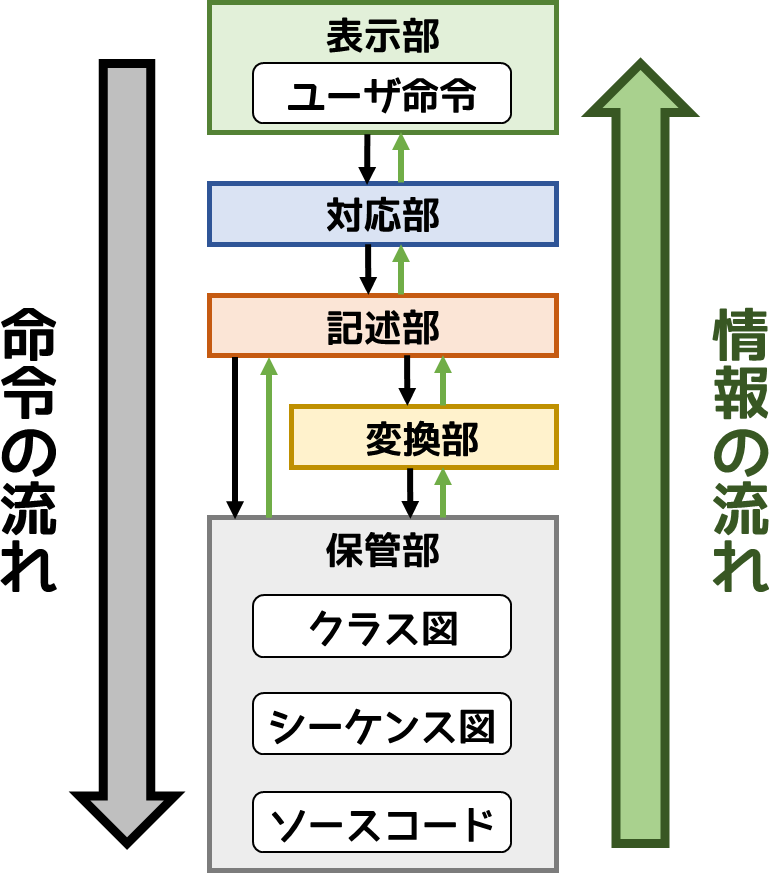
\includegraphics[keepaspectratio, width=160mm]{figs/retussStructure}
	\caption{\tool{}の構造とデータ遷移}
	\label{fig:toolStructure}
\end{figure}

% 適用例
\chapter{適用例}\label{cha:Indication}

% 考察
\chapter{考察}\label{cha:Evaluation}

% おわりに
\chapter{おわりに} \label{cha:Conclusion}

%%
% 謝辞
%
\acknowledgment{}

本研究において、数多くのアドバイス、叱咤激励、そして知識をいただきました、宮崎大学工学教育研究部の片山徹郎教授に、心から感謝申し上げます。
教授就任、おめでとうございます。

また、本論文の執筆にあたり、時にはユーモアを交え、貴重なご意見とご指摘をいただきました、宮崎大学工学教育研究部の伊達章准教授と油田健太郎准教授に、深く感謝いたします。

そして、\tool{}の拡張を名乗り上げてくれた栗原氏、ならびに協力してくださった株式会社スカイコムの皆様、ありがとうございます。
卒論を完成させてくれること、期待します。

なにより、研究の相談、実験の手伝い、話し相手など、私と仲良くしてくださった研究室のメンバー、今までありがとうございます。
特に、締切直前の実験のお手伝いをしてくださった、平木場氏、宮地氏、執行氏、中村氏、楢木氏、原田氏、以上6名の皆様、助かりました。

最後に、私の心の支えとなってくれた多くの方々、本当にありがとうございました。
6年間、楽しい大学生活と研究生活を過ごすことができました。


%%
% 参考文献
%
\begin{thebibliography}{99}
  \bibitem{米国におけるIoT} 八山 幸司 著: ``米国におけるIoT(モノのインターネット)に関する取り組みの現状,'' IPA New York, 2015
  
  \bibitem{通商白書2016} 経済産業省: ``通商白書2016,'' 経済産業省, 2016
  
  \bibitem{JAXAソフトウェアエンジニアリング} JAXA 研究開発部門 第三研究ユニット: ``ソフトウェアエンジニアリング,'' http://stage.tksc.jaxa.jp/jedi/devel/index.html (最終アクセス 2019/01/25)
  
  \bibitem{みずほシステム障害} 失敗知識データベース: ``みずほフィナンシャルグループ大規模システム障害,'' http://www.shippai.org/fkd/cf/CA0000623.html (最終アクセス 2019/01/25)
  
  \bibitem{ソフトウェア開発の定量化手法} Capers Jones 著, 富野 壽, 小坂 恭一 監訳: ``ソフトウェア開発の定量化手法 -生産性と品質の工場を目指して- 第3版,'' 共立出版, 2010
  
  \bibitem{SQuBOK} SQuBOK策定部会: ``ソフトウェア品質知識体系ガイド 第2版,'' オーム社, 2014
  
  \bibitem{REBOK} 情報サービス産業協会: ``要求工学知識体系,'' 近代科学社, 2011
  
  
  % 森氏の成果物
  \bibitem{九州支部} 森 敬介, 片山 徹郎: ``UMLとソースコード間でリアルタイムにトレーサビリティを維持するツールRETUSSについて,'' 平成29年度 電気・情報関係学会九州支部連合大会, pp. 104--105, 2017
  
  \bibitem{ICAROB2018} Keisuke Mori, Tetsuro Katayama, Yoshihiro Kita, Hisaaki Yamaba, Kentaro Aburada, and Naonobu Okazaki : ``Implementation of RETUSS to Ensure Traceability between Class Diagram in UML and Java Source Code in Real Time,'' The 2018 International Conference on Artificial Life and Robotics (ICAROB2018), pp. 522--525, 2018
  
  \bibitem{紀要} 森 敬介, 片山 徹郎: ``UMLとソースコードの間でトレーサビリティをリアルタイムに維持するツールRETUSSの現状と課題,'' 宮崎大学工学部紀要 第47号, pp. 343--347, 2018
  
  \bibitem{JRNAL} Tetsuro Katayama, Keisuke Mori, Yoshihiro Kita, Hisaaki Yamaba, Kentaro Aburada, Naonobu Okazaki: ``RETUSS: Ensuring Traceability System between Class Diagram in UML and Java Source Code in Real Time,'' Journal of Robotics, Networking and Artificial Life, Vol. 5(2), pp. 114--117, 2018
  
  \bibitem{RETUSS} GitHub: ``RETUSS: Real-time Ensure Traceability between UML and Source-code System,'' https://github.com/Morichan/Retuss (最終アクセス 2019/01/25)
  
  
  \bibitem{UML} UML (Unified Modeling Language): http://www.uml.org/ (最終アクセス 2019/01/25)
  
  \bibitem{UML2.0仕様書} Object Management Group 著, 西原 祐善 監訳: ``UML2.0仕様書 2.1対応,'' オーム社, 2006
  
  \bibitem{UML2.0クイックリファレンス} Dan Pilone, Neil Pitman 著, 原 隆文 訳: ``UML2.0クイックリファレンス,'' オライリー・ジャパン, 2008
  
  \bibitem{OMG} OMG (Object Management Group): http://www.omg.org/ (最終アクセス 2019/01/25)
  
  
  % 森氏の成果物
  \bibitem{ICAROB2019} Keisuke Mori, Tetsuro Katayama, Yoshihiro Kita, Hisaaki Yamaba, Kentaro Aburada, and Naonobu Okazaki: ``Development of Library Fescue Extracting Elements of Attributes and Operations of Class Diagram in UML,'' The 2019 International Conference on Artificial Life and Robotics (ICAROB2019), pp. 165--168, 2019
  
  \bibitem{Fescue} GitHub: ``Fescue: Feature Elements Section of Class in UML Extraction,'' https://github.com/Morichan/Fescue (最終アクセス 2019/01/25)
  
  
  \bibitem{プログラミング言語Java} Ken Arnold, James Gosling, David Holmes 著, 柴田 芳樹 訳: ``プログラミング言語Java 第4版,'' 東京電機大学出版局, 2014
  
  \bibitem{Java9} Oracle: ``Java Platform, Standard Edition 9 Reference Implementations,'' http://jdk.java.net/java-se-ri/9 (最終アクセス 2019/01/25)
  
  \bibitem{ISO9000} ISO TC176/SC1: ``ISO 9000:2005,'' International Organization for Standardization, 2005
  
  \bibitem{ANTLR4Reference} Terence Parr 著: ``The Definitive ANTLR 4 Reference,'' Pragmatic Bookshelf, 2013
  
  \bibitem{ANTLR} ``ANTLR,'' http://www.antlr.org/ (最終アクセス 2019/01/25)
  
  \bibitem{antlr4github} GitHub: ``ANTLR v4,'' https://github.com/antlr/antlr4 (最終アクセス 2019/01/25)
  
  \bibitem{ISO14977} ISO JTC1/SC22: ``ISO 14977:1996,'' International Organization for Standardization, 1996
  
  \bibitem{grammars-v4github} GitHub: ``grammars-v4,'' https://github.com/antlr/grammars-v4 (最終アクセス 2019/01/25)
  
  \bibitem{JUnit5} The JUnit Team: JUnit 5, https://junit.org/junit5/ (最終アクセス 2019/01/25)
  
  \bibitem{Jacoco} EclEmma 3.1.1: EclEmma - JaCoCo Java Code Coverage Library, https://www.jacoco.org/jacoco/ (最終アクセス 2019/01/25)
  
  \bibitem{ソフトウェアテスト} 高橋 寿一: 知識ゼロから学ぶソフトウェアテスト 改訂版, 翔泳社, 2013
  
  \bibitem{TravisCI} Travis CI: Travis CI - Test and Deploy Your Code with Confidence, https://travis-ci.org/ (最終アクセス 2019/01/25)
  
  \bibitem{astah} astah*: ``Astah - Software Design Tools for Agile teams with UML, ER Diagram, Flowchart, Mindmap and More \textbar{} Astah.net,'' http://astah.net/ (最終アクセス 2019/01/25)
  
  \bibitem{BlueJ} Michael Kolling and Bruce Quig: ``The BlueJ system and its pedagogy,'' Computer Science Education, Vol. 13, No. 4, pp. 208--213, 2014
  
  \bibitem{表入力によるJava} 湯浅 正徳, 梅澤 大志, 今野 俊直, 吉田 信一朗, 渡辺 康之, 紫合 治: ``表入力によるJAVAプログラムの設計支援ツール,'' 情報処理学会第74回全国大会講演論文集, Vol. 2012, No. 1, pp. 321--322, 2012
  
  \bibitem{EA} SPARX SYSTEMS: ``UML/SysMLモデリングツール Enterprise Architect(エンタープライズ アーキテクト) - EA,'' https://www.sparxsystems.jp/ (最終アクセス 2019/01/25)
  
  \bibitem{Visual Paradigm} Visual Paradigm: ``Ideal Modeling \& Diagramming Tool for Agile Team Collaboration,'' https://www.visual-paradigm.com/ (最終アクセス 2019/01/25)
  
  \bibitem{PlantUML} PlantUML: ``シンプルなテキストファイルでUMLが書ける、オープンソースのツール,'' http://plantuml.com/ (最終アクセス 2019/01/25)
  
  \bibitem{UMLetPaper} M. Auer, T. Tschurtschenthaler and S. Biffl: ``A Flyweight UML Modelling Tool for Software Development in Heterogeneous Environments,'' Proc. 29th Conference on EUROMICRO, p. 267, 2003
  
  % 以降の既存のツールは消してもいいでしょ......載せるけど!
  \bibitem{UMLet} UMLet: ``UMLet - Free UML Tool for fast UML Diagrams,'' https://www.umlet.com/ (最終アクセス 2019/01/25)
  
  \bibitem{AnchorGardenPlus} 浅井 俊伍, 酒井 三四郎: ``オブジェクト指向言語における主要な概念を理解するためのワークベンチ,'' 情報教育シンポジウム2015論文集, Vol. 2015, pp. 1--8, 2015
  
  \bibitem{Green} green: ``Green UML :: Home Page,'' http://green.sourceforge.net/index.html (最終アクセス 2019/01/25)
  
  \bibitem{Amateras} Project Amateras; enjoy your development: ``AmaterasUML - Project Amateras,'' http://amateras.osdn.jp/cgi-bin/fswiki/wiki.cgi?page=AmaterasUML (最終アクセス 2018-07-30)
  
  % HTTP ERROR 404 in 2019/01/25
  \bibitem{Poseidon} gentle ware: ``Gentleware - model to business: poseidon for uml 8.0 beta,'' http://www.gentleware.com/new-poseidon-for-uml-8-0.html (最終アクセス 2018-07-30)
  
  \bibitem{1stModeller} TOM'S SOFTWARE: ``1st Modeller (UMLモデリングツール),'' http://hp.vector.co.jp/authors/VA017111/ (最終アクセス 2019/01/25)
  
  \bibitem{PatternWeaver} Technologic Arts Co., Ltd.: ``パターンウィーバー:パターンウィーバー,'' http://pw.tech-arts.co.jp/ (最終アクセス 2019/01/25)
  
  \bibitem{Umbrello} KDE e.V.: ``Umbrello Project - Welcome to Umbrello - The UML Modeller,'' https://umbrello.kde.org/ (最終アクセス 2019/01/25)
  
  \bibitem{Violet} Cay S. Horstmann and Alexandre de Pellegrin: ``Violet UML Editor : easy to use, completely free,'' http://alexdp.free.fr/violetumleditor/page.php (最終アクセス 2019/01/25)
  
  \bibitem{DiaDiagram} dia-installer.de: ``Dia draws your structured diagrams: Free Windows, Mac OS X and Linux version of the popular open source program,'' http://dia-installer.de/ (最終アクセス 2019/01/25)
\end{thebibliography}

%%
% 付録
%
% \appendix{} % 付録は基本的に使わない

\end{document}
